\section{LabVIEW Saving and Reading \label{sec-saveread}}  

This tutorial is to give you a sense of how to save and read data within
LabVIEW.  Saving data is reasonably straight forward.  You create a VI, and use
a ``Collector'' to collect all the data during the simulation/experiment.  Then
you must use ``Unbundle By Name'' and put all the data you want to save into the
same array by using ``Build Array.''  Lastly, the ``Write File To Spreadsheet''
utility will allow you to write the file in a convenient format.  (All this is
shown in Fig.\ref{fig-savedata}.)  Note that you \emph{must} allow the
simulation to finish or data will not be written to the file.  Also note
that LabVIEW allows you to plot multiple plots on the same graph, as shown.

\begin{figure}[h!]
\centering
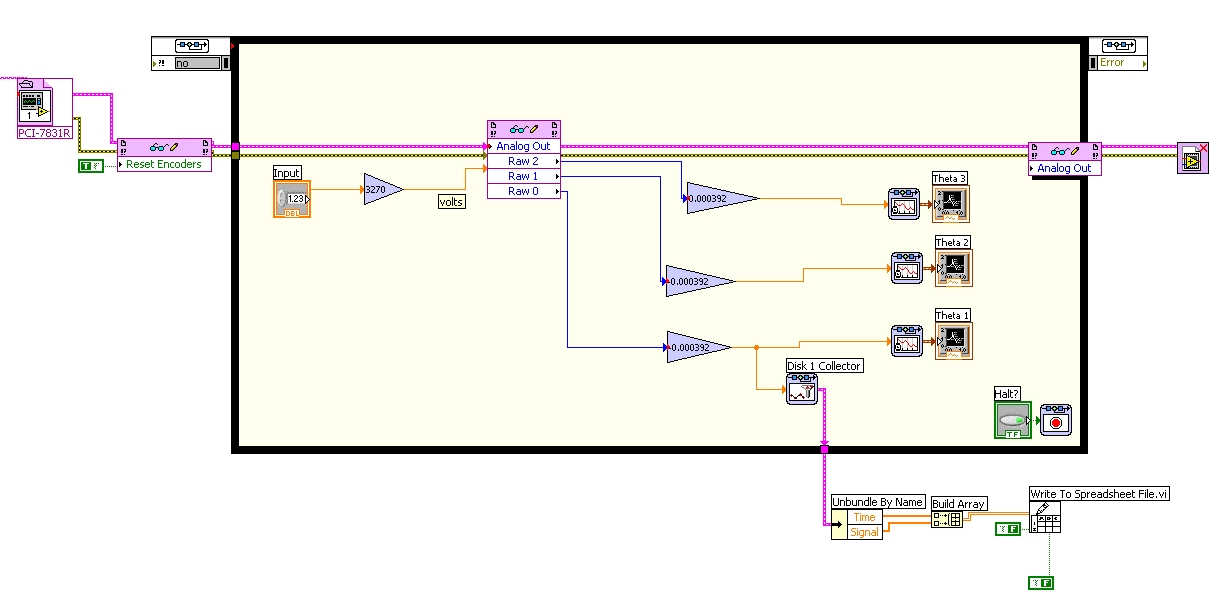
\includegraphics[width=6in]{saveread/write1}
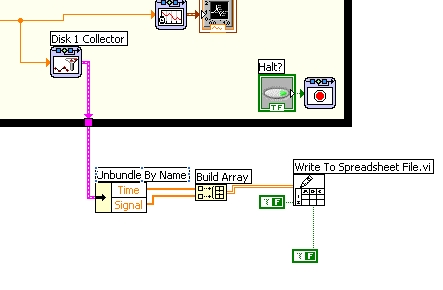
\includegraphics[width=5in]{saveread/write2}
\caption{(top) A VI  that saves data from an FPGA, (bottom) an enlargment of the section of
  code that saves data}
\label{fig-savedata}
\end{figure}


Now, reading data is similarly straight forward.  Assuming that you have saved
the data as above (in a spreadsheet format), you can use the ``Read From
Spreadsheet'' utility.  The data will be in an array format already, but you
must use the ``Index Array'' to select the data.  Figure~\ref{fig-readdata1}
shows the use of the ``Index Array'' block to select the first (``0''th) and
second (``1''st) signals from the data.  These can then either be used or
bundled together and plotted.

\begin{figure}[h!]
\centering
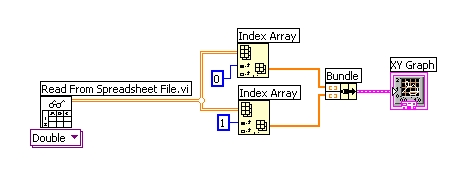
\includegraphics[width=5in]{saveread/read1}
\caption{A VI that reads data}
\label{fig-readdata1}
\end{figure}

%\begin{figure}[h!]
%\centering
%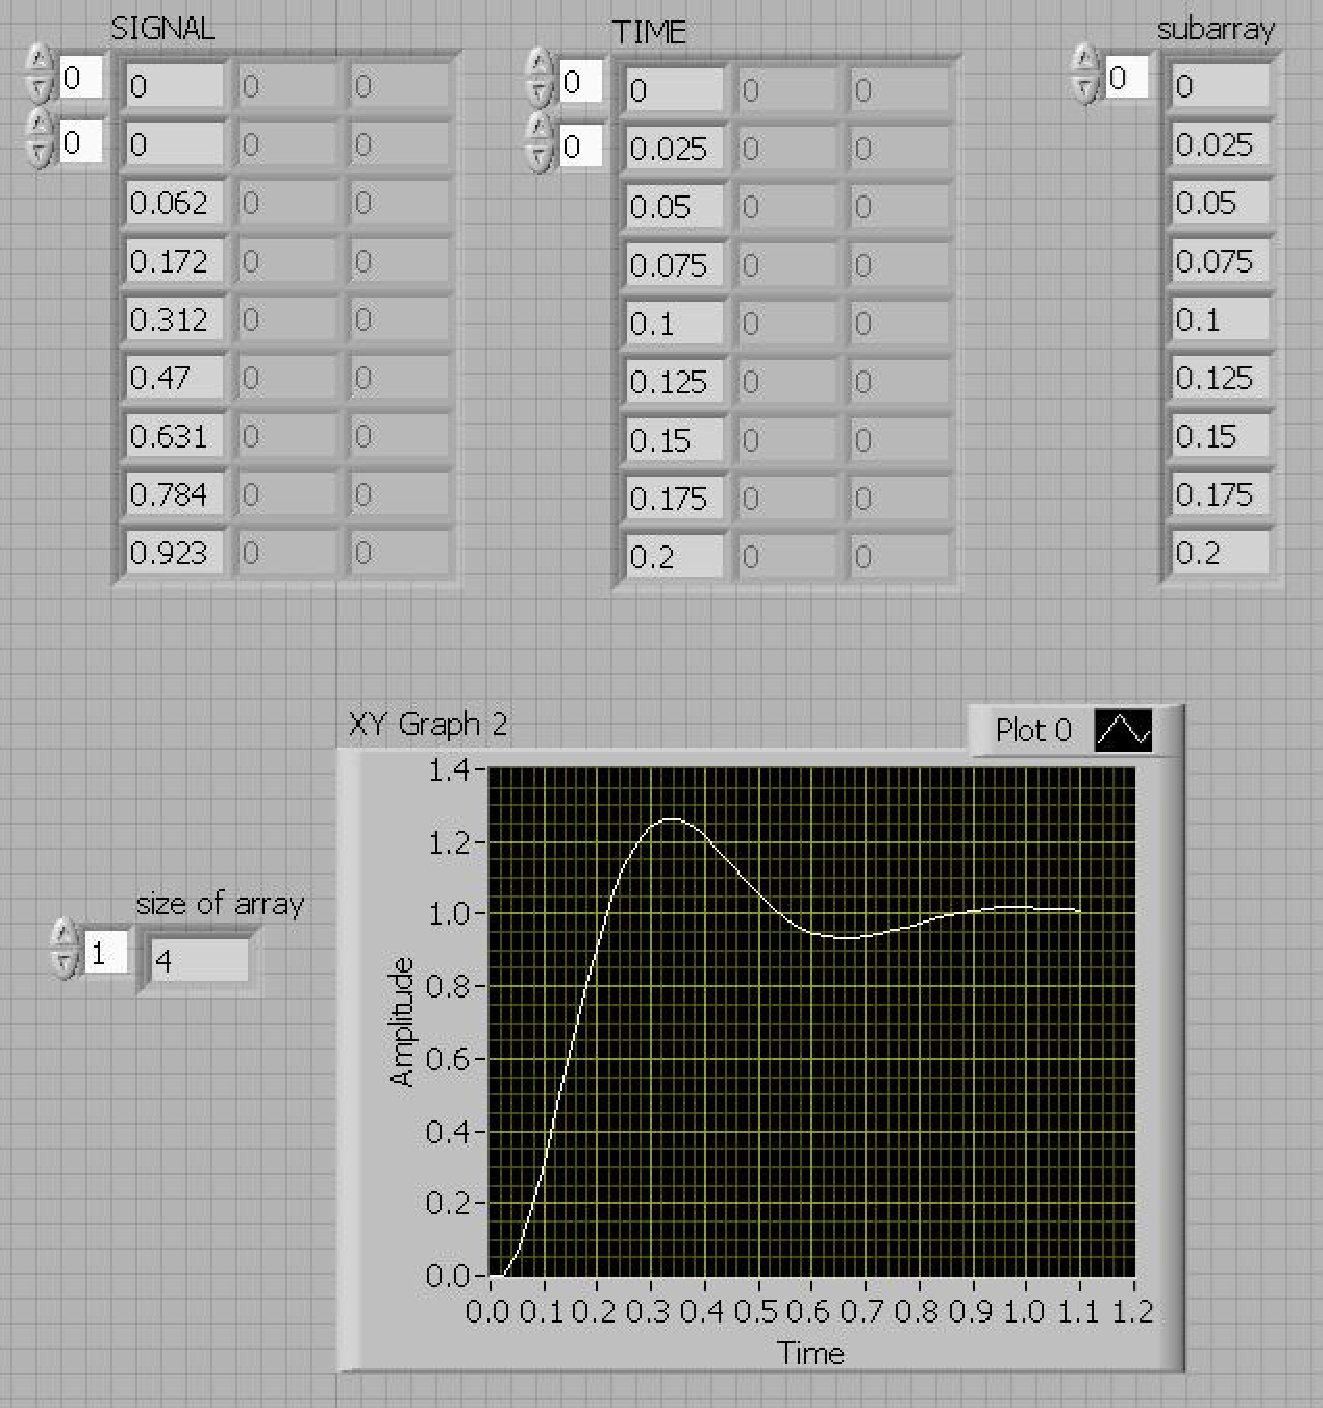
\includegraphics[width=3in]{saveread/readdata3}
%\caption{The Front Panel of the VI that reads data}
%\label{fig-readdata2}
%\end{figure}

%\newpage

%% Local Variables:
%% TeX-master: "../LVmanual.tex"
%% End:

